%%
%% This is file `sample-sigplan.tex',
%% generated with the docstrip utility.
%%
%% The original source files were:
%%
%% samples.dtx  (with options: `sigplan')
%% 
%% IMPORTANT NOTICE:
%% 
%% For the copyright see the source file.
%% 
%% Any modified versions of this file must be renamed
%% with new filenames distinct from sample-sigplan.tex.
%% 
%% For distribution of the original source see the terms
%% for copying and modification in the file samples.dtx.
%% 
%% This generated file may be distributed as long as the
%% original source files, as listed above, are part of the
%% same distribution. (The sources need not necessarily be
%% in the same archive or directory.)
%%
%% Commands for TeXCount
%TC:macro \cite [option:text,text]
%TC:macro \citep [option:text,text]
%TC:macro \citet [option:text,text]
%TC:envir table 0 1
%TC:envir table* 0 1
%TC:envir tabular [ignore] word
%TC:envir displaymath 0 word
%TC:envir math 0 word
%TC:envir comment 0 0
%%
%%
%% The first command in your LaTeX source must be the \documentclass command.
%%\documentclass[sigplan,screen]{acmart}
\documentclass[sigconf,review,anonymous,nonacm=true]{acmart}
% \documentclass[sigplan,screen]{acmart}
% \usepackage{cite}
\usepackage{graphicx}
\graphicspath{ {images/} }
\usepackage{tabularx}
\usepackage{mdframed}

%% NOTE that a single column version is required for 
%% submission and peer review. This can be done by changing
%% the \doucmentclass[...]{acmart} in this template to 
%% \documentclass[manuscript,screen,review]{acmart}
%% 
%% To ensure 100% compatibility, please check the white list of
%% approved LaTeX packages to be used with the Master Article Template at
%% https://www.acm.org/publications/taps/whitelist-of-latex-packages 
%% before creating your document. The white list page provides 
%% information on how to submit additional LaTeX packages for 
%% review and adoption.
%% Fonts used in the template cannot be substituted; margin 
%% adjustments are not allowed.
%%
%% \BibTeX command to typeset BibTeX logo in the docs
\AtBeginDocument{%
  \providecommand\BibTeX{{%
    \normalfont B\kern-0.5em{\scshape i\kern-0.25em b}\kern-0.8em\TeX}}}


%% Rights management information.  This information is sent to you
%% when you complete the rights form.  These commands have SAMPLE
%% values in them; it is your responsibility as an author to replace
%% the commands and values with those provided to you when you
%% complete the rights form.
\setcopyright{acmlicensed}
\copyrightyear{2018}
\acmYear{2018}
\acmDOI{XXXXXXX.XXXXXXX}

%% These commands are for a PROCEEDINGS abstract or paper.
\acmConference[Conference acronym 'XX]{Make sure to enter the correct
  conference title from your rights confirmation emai}{June 03--05,
  2018}{Woodstock, NY}
%
%  Uncomment \acmBooktitle if th title of the proceedings is different
%  from ``Proceedings of ...''!
%
%\acmBooktitle{Woodstock '18: ACM Symposium on Neural Gaze Detection,
%  June 03--05, 2018, Woodstock, NY} 
\acmISBN{978-1-4503-XXXX-X/18/06}


%%
%% Submission ID.
%% Use this when submitting an article to a sponsored event. You'll
%% receive a unique submission ID from the organizers
%% of the event, and this ID should be used as the parameter to this command.
%%\acmSubmissionID{123-A56-BU3}

%%
%% For managing citations, it is recommended to use bibliography
%% files in BibTeX format.
%%
%% You can then either use BibTeX with the ACM-Reference-Format style,
%% or BibLaTeX with the acmnumeric or acmauthoryear sytles, that include
%% support for advanced citation of software artefact from the
%% biblatex-software package, also separately available on CTAN.
%%
%% Look at the sample-*-biblatex.tex files for templates showcasing
%% the biblatex styles.
%%

%%
%% The majority of ACM publications use numbered citations and
%% references.  The command \citestyle{authoryear} switches to the
%% "author year" style.
%%
%% If you are preparing content for an event
%% sponsored by ACM SIGGRAPH, you must use the "author year" style of
%% citations and references.
%% Uncommenting
%% the next command will enable that style.
%%\citestyle{acmauthoryear}

%%
%% end of the preamble, start of the body of the document source.
\begin{document}

%%
%% The "title" command has an optional parameter,
%% allowing the author to define a "short title" to be used in page headers.
\title{Are Causal Inference Algorithms really stable?}

%%
%% The "author" command and its associated commands are used to define
%% the authors and their affiliations.
%% Of note is the shared affiliation of the first two authors, and the
%% "authornote" and "authornotemark" commands
%% used to denote shared contribution to the research.
\author{Aoishi Das}
\email{adas23@ncsu.ed}
\affiliation{%
  \institution{North Carolina State University, Department of Computer Science}
}

\author{Dr. Timothy Menzies}
\email{timm@ieee.org}
\affiliation{%
  \institution{North Carolina State University, Department of Computer Science}
}


%%
%% By default, the full list of authors will be used in the page
%% headers. Often, this list is too long, and will overlap
%% other information printed in the page headers. This command allows
%% the author to define a more concise list
%% of authors' names for this purpose.


%%
%% The abstract is a short summary of the work to be presented in the
%% article.
\begin{abstract}
  In today's world, Artificial Intelligence and Machine Learning is consolidating it's impact in almost every sector. Hence Data is and must be considered the new gold. But the biggest challenge in itself is collecting that huge amount of data required to satiate those Machine Learning models. The solution: Why wait for Data? Why not synthesize it? Generating synthetic data seems to be a really good option since it would create all the data needed for the data hungry machine learning algorithms, enable data sharing and increase data security especially when working with sensitive data. Amidst all these an important question arises: Is the synthetic data on which we are going to train our Machine Learning models correct? Are the Data Synthesizing algorithms able to truly capture the essence and nature of the original data and replicate that? Are the algorithms used to study the causal relationship in the original data stable? In this paper we performed an extensive study to understand the prior works involving frequently used causal graph generators like FCI(Fast Causal Inference), Granger Causality, Bayesian Networks, Root Cause Analysis. Jaccard Coefficient was used to compare the similarity of two causal graphs. We then experimented extensively with GFCI(Greedy Fast Causal Inference) using Tetrad\cite{TTT}. We performed multiple experiments to study how using different combination of hyperparameters like number of bootstrapping iterations, seed, etc can affect the stability of causal graphs. 
\end{abstract}

%%
%% The code below is generated by the tool at http://dl.acm.org/ccs.cfm.
%% Please copy and paste the code instead of the example below.
%%

\begin{CCSXML}
<ccs2012>
   <concept>
       <concept_id>10002950.10003624.10003633</concept_id>
       <concept_desc>Mathematics of computing~Graph theory</concept_desc>
       <concept_significance>500</concept_significance>
       </concept>
   <concept>
       <concept_id>10011007.10011074.10011134.10003559</concept_id>
       <concept_desc>Software and its engineering~Open source model</concept_desc>
       <concept_significance>300</concept_significance>
       </concept>
   <concept>
       <concept_id>10003752.10003809.10003635</concept_id>
       <concept_desc>Theory of computation~Graph algorithms analysis</concept_desc>
       <concept_significance>300</concept_significance>
       </concept>
 </ccs2012>
\end{CCSXML}

\ccsdesc[500]{Mathematics of computing~Graph theory}
\ccsdesc[300]{Software and its engineering~Open source model}
\ccsdesc[300]{Theory of computation~Graph algorithms analysis}


%%
%% Keywords. The author(s) should pick words that accurately describe
%% the work being presented. Separate the keywords with commas.
\keywords{causality, software analytics, stability}

%% A "teaser" image appears between the author and affiliation
%% information and the body of the document, and typically spans the
%% page.
% \begin{teaserfigure}
%   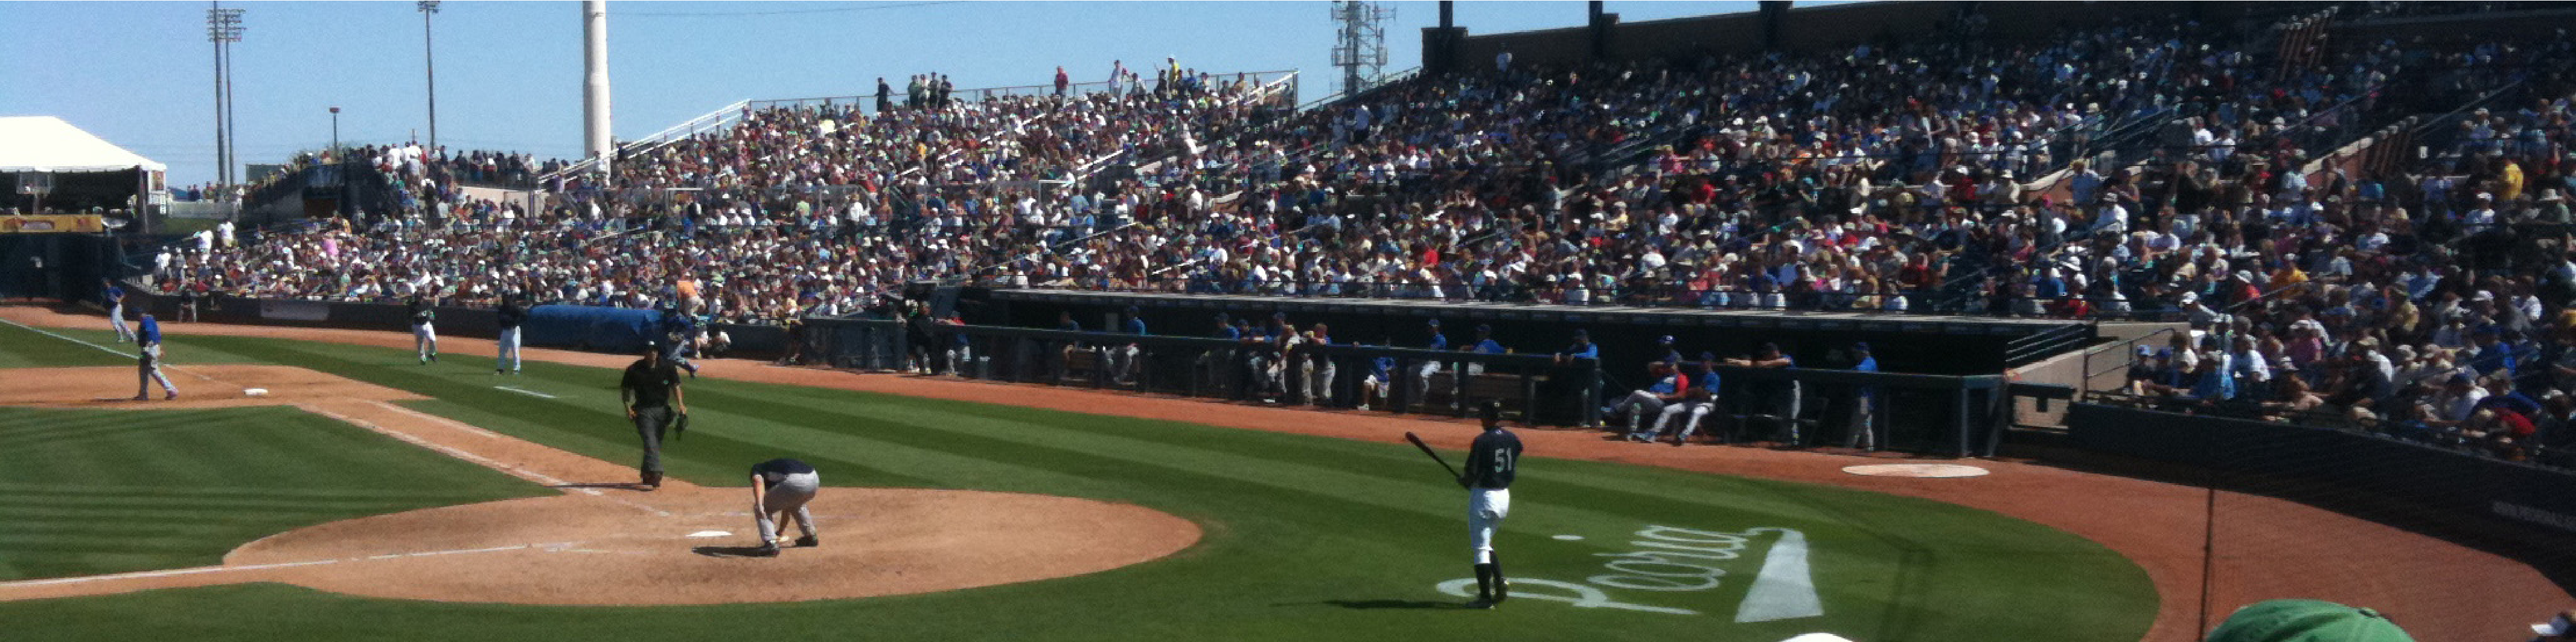
\includegraphics[width=\textwidth]{sampleteaser}
%   \caption{Seattle Mariners at Spring Training, 2010.}
%   \Description{Enjoying the baseball game from the third-base
%   seats. Ichiro Suzuki preparing to bat.}
%   \label{fig:teaser}
% \end{teaserfigure}

\received{20 February 2007}
\received[revised]{12 March 2009}
\received[accepted]{5 June 2009}

%%
%% This command processes the author and affiliation and title
%% information and builds the first part of the formatted document.
\maketitle

\section{Introduction}
Generating data for Machine Learning models is for sure a gigantic and quite tricky task. The data that is already available for model training might also not be very good due to a lot of factors like missing values, limited number of data points, low quality data. Data synthesizers seems to be the best choice since it can generate lots of data that also ensures security and ease of data sharing. Most of the data synthesizers apply different Causal inference algorithms like GFCI (Greedy Fast Causal Interference), Greedy Bayes Algorithm to determine the correlation among attributes which in turn is used to generate the data summary. New data is generated based on this model summary. Hence it is very important that the correlation relations learned by the Causal Inference algorithms are correct since modeling the new data largely depends on that.\\
One pressing issue has been found across majority of these data synthesizers. Most of them do not check for the stability of the correlations (could be represented using causal graphs) generated by causal inference algorithms. In this paper we will talk about our findings that show how many of these causal graphs have been found to vary depending on the combination of hyperparameters used while modeling that graph, The biggest challenge in that scenario is 
\begin{itemize}
    \item How do we choose which graph best represents the causal relationship in the data?
    \item Which causal representation should be chosen while deriving the data summary and hence subsequently generating the synthesized data? 
\end{itemize} 
Thus, prior to modeling data based on these causal relations it needs to be ensured that the causal relationship used is the one that best represents the correlations that exist in the data.\\
To structure this analysis we ask three important questions:\\
\textbf{RQ1: Which are the most commonly used causal graph generation algorithms used to depict the correlation among attributes?}\\
Here we perform an extensive literature review to study about the various causal graph generation methods that have been used in Software Engineering related tasks. We also evaluated if these methods did take into consideration the stability of the generated causal graphs, To our surprise we found that none of these papers really talked about checking for stability of causal graphs.\\
\textbf{RQ2:How the combination of various hyperparameters affect the casual graphs?}\\
We experimented on changing some basic hyperparameters and study the effect of various combinations on the stability of the causal graphs. We experimented by changing seeds, number of bootstrap iterations and the versions of the dataset. Jaccard coefficient was used as a measure to check similarity between two graphs. \\
\textbf{RQ3:Does the size of the data affect the stability of the causal graphs? Will increasing the size of the dataset by generating data points and then generating causal graphs help in stabilizing them?}\\
Going through the outcome we were quite startled to find that changing the just a few hyperparameters made the graphs highly unstable. We wanted to check if the fact that some of these datasets were small in size might have an effect on the stability of the graph. Hence we generated synthetic data using the HOWSO algorithm and applied the same combination of hyperparamers if that improved the situation.  \\
\section{Related Work}
Data Synthesizing has been in the forefront over the past couple of years since it can mitigate the high demand of data needed to train Machine Learning models. One important criteria for the generated data is that it should be able to capture the nature and distribution of the real data as our models would be trained on these synthetic data. Hence we would want the data to be as close as possible to the real data. The data synthesizer algorithm\cite{DS} proposed adopts three high-level modules — DataDescriber, DataGenerator and ModelInspector. This paper provides an excellent approach to generate data by:
\begin{itemize}
    \item First by investigating the data types, correlations and distributions of the attributes and generating a data summary
    \item Next the DataGenerator samples from the summary and generate synthetic data
    \item The ModelInspector provides a comparative analysis of the two data to show it's accuracy.
\end{itemize}The DataDescriber uses the GreedyBayes algorithm to construct Bayesian networks (BN) to model correlated attributes. This prompted us to check if the Bayesian Network generated is prone to change with respect to hyperparameters. On varying basic hyperparameters like seed, degree of Bayesian Network it results in significantly different causal graphs with Jaccard coefficient ranging as low as 0.11. This prompted us to check out other common causal graph generators used to solve Software Engineering problems.\\
Causality has been a crucial component in understanding the correlations among attributes and has been widely implemented to solve numerous problems in Software Engineering domain:
\begin{itemize}
    \item Software engineering problems are interrelated causally through software processes and it is valuable to study the causalities as it can help to prevent software project failures \cite{Per} where they performed Root Cause Analysis\cite{P2} to identify the causes of selected software failures.
    \item Applying causality in Fairness Testing: Testing software for Discrimination.\cite{FT}  Software testing offers a unique opportunity to conduct causal experiments to determine statistical causality where the software could be run on an input, modify a specific input characteristic and it can be observed if that modification causes a change in the output.
    \item A lot of work is going on to study the Statistical Causal Inference (SCI) Methods to estimate causal effects from Observational Data. \cite{Ap} Pearl's framework is one such causality inference model which has gained popularity recently. 
    \item Causality is even widely implemented to perform Software project risk analysis. The main idea is to apply Causal inference algorithms like Bayesian Networks with Causality Constraints\cite{BNCC} to identify the relationship between risk factors and project outcome.
    \item Apply Granger Causality Test to idetify causal relationships that exist in Time Series Data. In the paper "Competence-Confidence Gap: A Threat to Female Developers’ Contribution on GitHub"\cite{CC}, the authors explored how the competence-confidence gap is a threat to female developers’ contribution on GitHub. 
\end{itemize}
Hence a wide range of fields in Software Engineering has applied different Causality inference algorithms to understand the causal relationships between factors. However one common issue noticed is the lack of any algorithm that checks for the stability of the generated causal graphs. The burning question still persists : How do we ensure that the causal graph generated is the one that represents the data best? 
\section{Experimental Setup}
To find an answer to all these questions, we have performed some experiments to see if the commonly used and popular causal graph generators, result in stable graphs. The dataset used is from the TeraPromise-Defect-Dataset\cite{DT}. We used different versions of mainly 4 types of dataset from the ck folder. 
\begin{itemize}
    \item ant 
    \item camel
    \item synapse
    \item ivy
\end{itemize}
Refer to Table \ref{tab:attributes} which gives a detailed description of the attributes\cite{D} of the dataset.

\begin{table}[h]
\centering
\caption{Description of Attributes}
\label{tab:attributes}
\begin{tabular}{|l|p{7cm}|} % Adjust the 8cm as needed
\hline
\textbf{Attribute} & \textbf{Description} \\ \hline
wmc & Weight Method Class or McCabe's complexity: Counts branch instructions in a class. \\ \hline
dit & Depth Inheritance Tree: Counts the number of "fathers" a class has. \\ \hline
noc & Number of Children: Counts the number of immediate subclasses. \\ \hline
cbo & Coupling between objects: Counts the number of dependencies a class has. \\ \hline
rfc & Response for a Class: Counts unique method invocations in a class. \\ \hline
lcom & Lack of Cohesion of Methods: Calculates LCOM metric. \\ \hline
ca & Afferent Couplings that measures the number of classes that depend on a given class. \\ \hline
ce & Efferent couplings that counts the number of classes that a given class depends on\\ \hline
npm & Number of Public methods that counts the number of public methods. \\ \hline
lcom3 & LCOM* (Lack of Cohesion of Methods): Modified version of LCOM. \\ \hline
loc & Lines of code: Counts the lines of code, ignoring empty lines and comments. \\ \hline
dam & Data Access Metric is the ratio of the number of private attributes to the total number of attributes declared in the
class. \\ \hline
moa & Measure of Aggregation that counts the number of data declarations (like class-level variables) whose types are user-defined classes. It represents the class's composition level.\\ \hline
mfa & Measure of Functional Abstraction that calculates the ratio of inherited methods to the total number of methods. It indicates how much a class is abstracting functionality.\\ \hline
cam & Cohesion Among Methods of Class) that measures the similarity of parameter lists of methods in a class, indicating method cohesion.\\ \hline
ic & Inheritance Coupling that counts the number of parent classes to which a class is coupled. It indicates the class's dependency on inherited methods.\\ \hline
cbm & Coupling Between Methods - measures the total complexity of coupling between methods in a class.\\ \hline
amc & Average Method Complexity - calculates the average complexity of methods in a class. \\ \hline
max\_cc & Maximum Cyclomatic Complexity - determines the maximum cyclomatic complexity among the methods of a class. \\ \hline
avg\_cc & Average Cyclomatic Complexity- calculates the average cyclomatic complexity of methods in a class. \\ \hline
bug & Number of bugs \\ \hline
\end{tabular}
\end{table}

For every dataset we wanted to explore if increasing the size of the data will result in increase in the stability of the causal graphs. For synthetic data generation we used the HOWSO Algorithm.

\subsection{HOWSO Algorithm}
Howso Engine is developed by Howso\footnote{https://www.howso.com/}. It is an AI engine which supports the synthetic data generation. Specifically, Howso Engine utilizes the k-nearest neighbors to synthesize data with both global and local distributions~\cite{howso}. The algorithm contains three parameters to control the search, and the best combination of the parameters is found by the grid search. Since there is only two parameters that need to be explored, the grid search is very fast.
\begin{itemize}
    \item The Minkowski coefficient $p \in [ 0.1, 2.0 ]$ which controls the calculation of distance.
        \begin{equation}
            d(x, y, \Delta) = (\sum_{i=1}^{n} \Delta(x_i, y_i)^p)^{1/p}
        \end{equation}
    \item Iteration parameter $l = 6$ which is used to find the parameter for distance calculation.
    \item The number of neighbors $k \in [5, 22]$ during the execution of $k$-nearest neighbors algorithm.
\end{itemize}

In the distance calculation, $\Delta$ is the specific function to measure the distance between two variables. Howso Engine implements the Lukaszyk-Karmowski metric (LK metric) for the Laplace distribution. Specifically,
\begin{equation}
    \Delta(x_i,y_i) = |x_j - x_i| + \frac{1}{2} e^{-\frac{|x_j - x_i|}{b}} \left( 3b+|x_j - x_i| \right)
\end{equation}
The Laplace distribution is preferred here since it makes entropy-minimizing assumptions about the underlying data, and more performant than Gaussian distribution. In the above calculation, $b$ is the surprisal that needs to be found through multiple iterations for each dataset. Specifically, the initial $b$ is set to $1/k$ where $k$ is the number of neighbors used in $k$-nearest neighbor algorithm. The first iteration finds the local neighbors by traditional Minkowski distance since no information in the initial round. In the end of the initial round, we can update the surprisal $b$:
\begin{itemize}
    \item For the numerical feature $k$, Howso Engine uses mean absolute deviation (MAE):
    \begin{equation}
        b = \frac{1}{n} \sum_{i=1}^{n} |x_i - \mu_k|
    \end{equation}
    \item For the symbolic feature, Howso Engine uses mode and accuracy instead of mean and MAE.
\end{itemize}

Once the value of $b$ is stabilized (which we found $b$ tends to stable in 6 iterations), Howso Engine iteratively picks one random feature to synthesize. Specifically,
\begin{itemize}
    \item The values in the first picked feature will be synthesized on the basis of the global histogram (for nominal features) or the global Laplace distribution (for continuous features).
    \item For all subsequent features, values are generated based on the distribution in the $k$ nearest neighbors to the partially synthesized cases.
\end{itemize}
The above process is done $m$ times per feature where $m$ is the number of synthetic instances that request to be generated.



In the above dataset there were three more attributes which were deleted due to the following reasons:
\begin{itemize}
    \item name : Had just the name of the dataset in all the columns
    \item version : Mentioned the version of the dataset, again had the same values in all rows
    \item name : Had unique values in all rows, hence wouldn't play a role in the correlation
\end{itemize}
For the Causal Graph generation we have used the Tetrad application \cite{TT}. It provides an excellent user friendly interface with a lot of different Causal Graph generation algorithms. It also allows the user to tune the hyperparameters.
We applied the GFCI (Greedy Fast Causal Inference)\cite{GFCI} to generate our causal graphs. Refer to Table \ref{hyp} for main hyperparameters that were tuned:

\begin{table}[h]
\centering
\caption{Hyperparameters tuned in GFCI}
\label{hyp}
\label{your-table-label}
\begin{tabular}{|p{5cm}|p{3cm}|}
\hline
Hyperparameter & Specifications \\ \hline
The number of bootstraps/resampling iterations & Minimum is 0 \\ \hline
The percentage of resample size & Minimum is 10\% \\ \hline
Seed for pseudo random number generator & Default value is -1 (off)\\ \hline
Should the original dataset be added as another bootstrapping & Default is Yes\\ \hline
Should sampling be done with replacement & Default is Yes \\ \hline
If individual bootstrapping graphs be saved & Default is Yes \\ \hline
\end{tabular}
\end{table}

\subsection{Synapse Dataset}
The details of the conditions used is shown in Table \ref{tab:conditions}\\
Figure \ref{synjacard} shows how the Jaccard coefficient varied for the Dataset: synapse. 


\begin{table}[h]
\centering
\caption{Comparison of Conditions for Synapse Dataset}
\label{tab:conditions}
\begin{tabularx}{0.5\textwidth}{|l|X|X|X|X|}
\hline
\textbf{Condition Number}                     & \textbf{1} & \textbf{2} & \textbf{3} & \textbf{4} \\ \hline
Dataset Version                      & 1.0          & 1.1          & 1.1          & 1.2          \\ \hline
Bootstraps                   & 0                    & 0                    & 5                    & 0                    \\ \hline
Percentage of Resamples     & 100                & 100               & 90                & 90                 \\ \hline
Seed                          & -1                   & -1                   & 3                    & 42                   \\ \hline
Add Original Dataset          & Y                    & Y                    & Y                    & N                    \\ \hline
Sampling with Replacement     & Y                    & Y                    & N                    & N                    \\ \hline
Save Individual Bootstrapping Graphs? & N                    & N                    & N                    & N                    \\ \hline
\end{tabularx}
\end{table}

\begin{figure}[h]
\caption{Synapse's Jaccard values.}\label{synjacard}
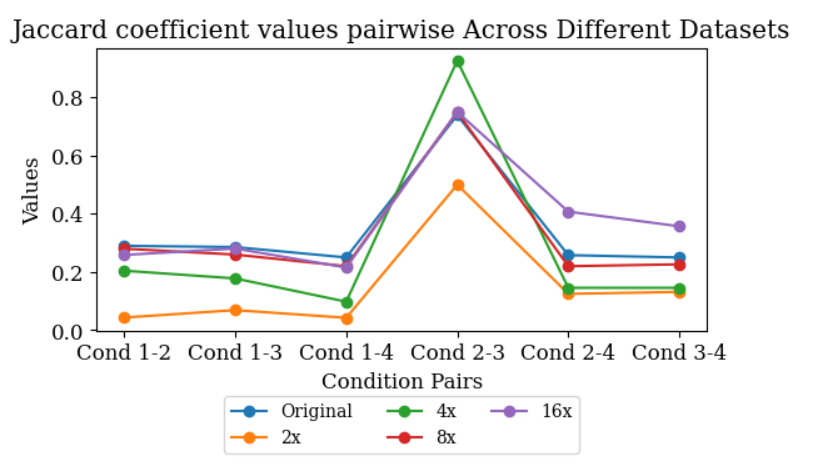
\includegraphics[width=9cm]{images/First_Pic.png}
\end{figure}

\subsection{Camel Dataset}
The details of the conditions used is shown in Table \ref{tab:conditions2}\\
Figure \ref{camjacard} shows how the Jaccard coefficient varied for the Dataset: camel. 


\begin{table}[h]
\centering
\caption{Comparison of Conditions for Camel dataset}
\label{tab:conditions2}
\begin{tabularx}{0.5\textwidth}{|l|X|X|X|X|X|}
\hline
\textbf{Condition Number} & \textbf{1} & \textbf{2} & \textbf{3} & \textbf{4} & \textbf{5} \\ \hline
Dataset version           & 1.0   & 1.2   & 1.4   & 1.4   & 1.6   \\ \hline
Bootstraps         & 0                & 1                & 0                & 5                & 0                \\ \hline
\% of Resamples    & 100            & 90             & 90             & 90            & 90            \\ \hline
Seed               & -1               & 42               & 3                & 42               & -1               \\ \hline
Add Orig. Dataset  & Y                & Y                & N                & Y                & N                \\ \hline
Sampling with Replacement     & Y                & Y                & N                & N                & N                \\ \hline
Save indiv. bootstrapping Graphs?  & N                & N                & N                & N                & N                \\ \hline
\end{tabularx}
\end{table}

\begin{figure}[h]
\caption{Camel's Jaccard values.}\label{camjacard}
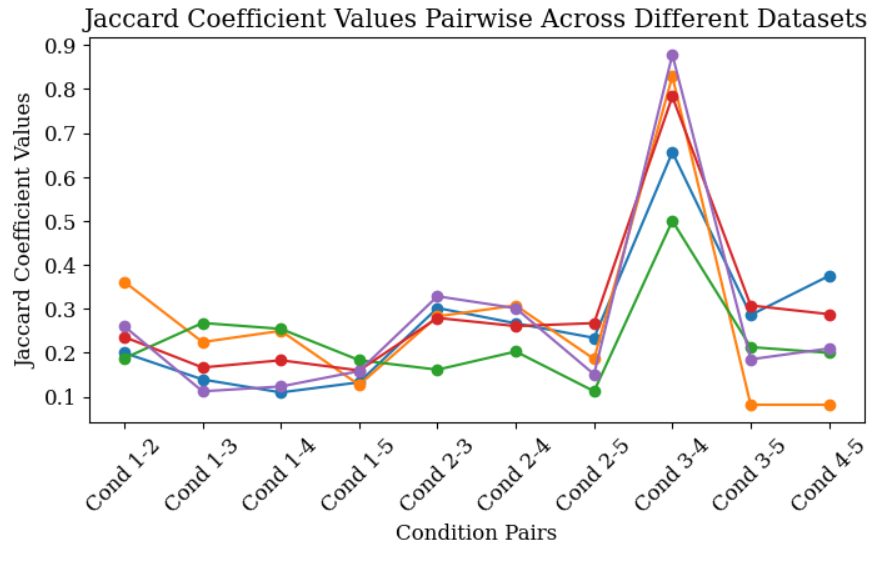
\includegraphics[width=9cm]{images/camel.png}
\end{figure}

\subsection{ant Dataset}
The details of the conditions used is shown in Table \ref{tab:conditions3}\\
Figure \ref{antjacard} shows how the Jaccard coefficient varied for the Dataset: ant. 

\begin{table}[h]
\centering
\caption{Comparison of Different Conditions for ant Dataset}
\label{tab:conditions3}
\begin{tabularx}{0.5\textwidth}{|l|X|X|X|X|X|X|}
\hline
\textbf{Condition Number}        & \textbf{1} & \textbf{2} & \textbf{3} & \textbf{4} & \textbf{5} & \textbf{6} \\ \hline
Dataset version                  & 1.3          & 1.4          & 1.5          & 1.6          & 1.7          & 1.7          \\ \hline
Bootstraps                & 0                & 5                & 0                & 2                & 5                & 2                \\ \hline
\% of Resamples           & 100            & 90            & 90            & 100            & 90            & 90            \\ \hline
Seed                      & -1          & 25               & 42               & -1          & 3                & 42               \\ \hline
Add Orig. Dataset         & Y                & Y                & N                & N                & N                & N                \\ \hline
Samp. w/ Repl.            & Y                & N                & Y                & N                & Y                & N                \\ \hline
Ind. Bootstrapping Graphs Saved?         & N                & N                & N                & N                & N                & N                \\ \hline
\end{tabularx}
\end{table}

\begin{figure}[h]
\caption{ant's Jaccard values.}\label{antjacard}
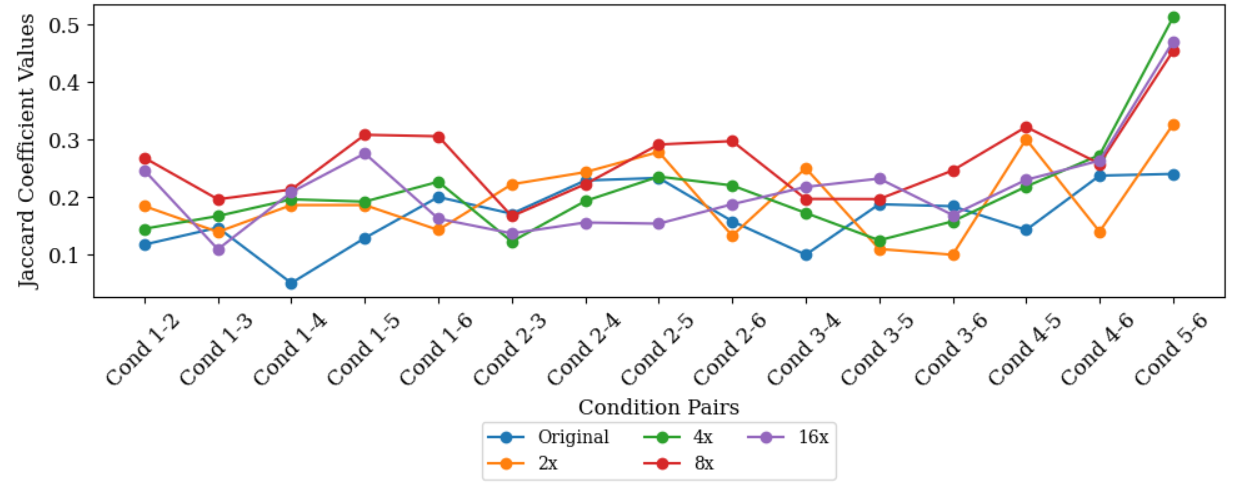
\includegraphics[width=9cm]{images/ant.png}
\end{figure}

\subsection{ivy Dataset}
The details of the conditions used is shown in Table \ref{tab:conditions4}\\
Figure \ref{ivyjacard} shows how the Jaccard coefficient varied for the Dataset: ivy. 

\begin{table}[h]
\centering
\caption{Comparison of Different Conditions for ivy Dataset}
\label{tab:conditions4}
\begin{tabularx}{0.5\textwidth}{|l|X|X|X|X|X|}
\hline
\textbf{Condition Number}        & \textbf{1} & \textbf{2} & \textbf{3} & \textbf{4} & \textbf{5}  \\ \hline
Dataset version                  & 1.1          & 1.1          & 1.4          & 1.4          & 2.0            \\ \hline
Bootstraps                & 0                & 10               & 5              & 5               & 5                \\ \hline
\% of Resamples           & 100            & 90            & 90            & 90            & 90                   \\ \hline
Seed                      & -1          & 42               & 42              & 3          & 3                        \\ \hline
Add Orig. Dataset         & Y                & Y                & N                & N                & N                        \\ \hline
Samp. w/ Repl.            & Y                & Y               & Y                & Y               & Y                \\ \hline
Ind. Bootstrapping Graphs Saved?         & N                & N                & N                & N                & N               \\ \hline
\end{tabularx}
\end{table}

\begin{figure}[h]
\caption{ivy's Jaccard values.}\label{ivyjacard}
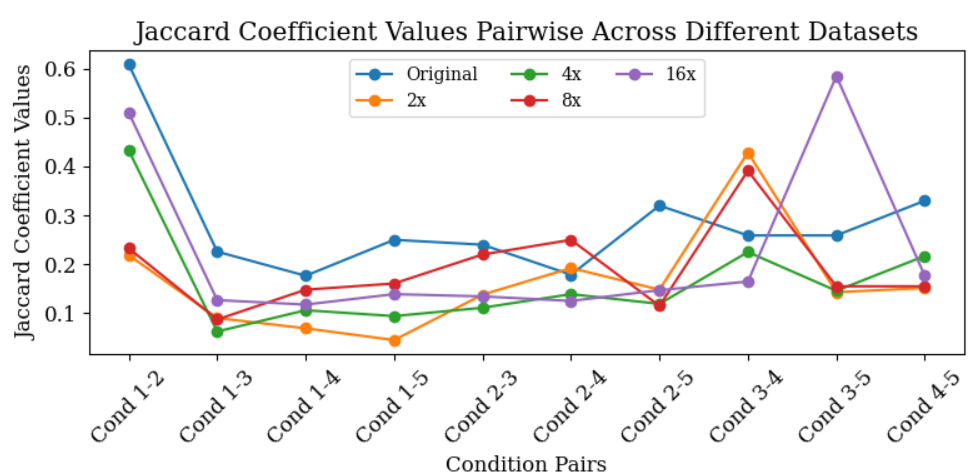
\includegraphics[width=9cm]{images/ivy.png}
\end{figure}

\section{Threat to Validity}
\textbf{Construct validity} is an issue with our parameter setting. In
this study, there were many parameter choices. Even after settling on one Causal Inference Algorithm - GFCI, there were still a lot of choices for Statistical Test like : DG LRT, Fisher Z test, Geberalized Information Criteria Score, KCI Test, MAG SEM BIC Test, Poisson Prior Test, SEM BIC Test and Uniform Scatter Test. There were other Score options as well like SEM BIC Score, CG-BIC, DG-BIC, EBIC Score etc. We chose Fisher Z Test and Sem BIC Test. Thus there is a possibility that there might be a more stable result if some other combination for Test and Score was chosen.\\
\textbf{Sample validity} threatens any study that reports conclusions from
learner L across data sets D for task using Test T and Score S . It
is quite possible that changing any of L, D, T and S would result in a
different conclusion. That said, at the very least, this study can say
that the the general trend observed using 3 different datasets remained the same with a poor Jaccard Coefficient across the cases.\\
\textbf{Conclusion validity}The use of Jaccard Coefficient to measure the similarity of causal graphs and the interpretation of these measurements could impact the validity of the conclusions drawn.

\section{CONCLUSION}
\textbf{RQ1: Which are the most commonly used causal graph generation algorithms used to depict the correlation among attributes?}\\

In thus study, we used a literature review to identify
commonly used causal graph generators. 

\vspace{2mm}
 \begin{mdframed}[backgroundcolor=gray!15,linewidth=3px,%
    rightline=false,% 
    topline=false,% 
    bottomline=false,] 
    \textbf{Ans}
According to the literature survey conducted, some of the most commonly used Causal graph generators were - Bayesian Network, Granger Causality, Feature Causality, GFCI (Greedy Fast Causal Inference) to name a few. However the highlight was that none of the papers really checked for the stability of the causal graphs generated.
\end{mdframed}
\vspace{2mm}

\textbf{RQ2:How the combination of various hyperparameters affect the casual graphs?}\\

Of the causal graph generators shown above, we focused
on one algorithm called \textbf{GFCI (Greedy Fast Causal Inference)} since this was used to solve a very similar kind of problem \cite{r14}. In that paper they aimed to propose an approach called CausalDefect to construct causal graph of defects, which provides a visual way to understand the causal
relationships between different features of defects. For that generator we observed:

\vspace{2mm}
 \begin{mdframed}[backgroundcolor=gray!15,linewidth=3px,%
    rightline=false,% 
    topline=false,% 
    bottomline=false,] 
\textbf{Ans}
Changing the hyperparameters had very large impact on the stability of the causal graphs, Most of the pair of causal graphs had very low Jaccard Coefficients (.3 or lower); i.e. they were very   dissimilarity.  Greatest instability was seen when changing
versions within one project.
\end{mdframed}
\vspace{2mm}

To say that another way, causal graphs are not definitive structures
describing core influences within a project. Rather, they suffer
from wild instability which means that conclusions reached in on version of the code (using causal graphs) probably do not hold for another version.

\textbf{RQ3:Does the size of the data affect the stability of the causal graphs? Will increasing the size of the dataset by generating data points and then generating causal graphs help in stabilizing them?}\\
\vspace{2mm}
 \begin{mdframed}[backgroundcolor=gray!15,linewidth=3px,%
    rightline=false,% 
    topline=false,% 
    bottomline=false,] 
\textbf{Ans:}
We had a theory in mind that maybe the amount of data has some relation with the stability. Since the datasets we experimented with has somewhat less number of data points we wanted to increase the dataset size and check if that has a positive effect on the stability of the graphs. Hence we used the HOWSO algorithm to generate some synthetic data of sizes - 2x, 4x, 8x and 16x. Unfortunately it didn't work out as we had envisioned. The behaviour was pretty erratic and there was no clear pattern across or even in the same dataset. 
\end{mdframed}
\vspace{2mm}

\section{Future Work}
As this work was at the verge of completion, we discovered a niche area of the literature exploring trust and causal graphs. While that discovery was too late to effect this work, it does presents promising line of future work. We came across another paper \cite{r15} that presents an interesting study about how sub sampling and sampling with replacement performed really well that could potentially serve as grounds for confidence in graph features.That paper experimented with a different algorithm and some different hyperparameter combinations.  This completely changed the course of our thoughts. In our approach we tried oversampling the data and check if that positively impacts the stability of the causal graph. However experimenting with sub sampling and resampling opens up a whole new area of conducting experiments and questions like
\begin{itemize}
    \item What other metrics are used to assess similarity among causal graphs?
    \item What other causal graph generators have been used and if those causal graph generation techniques might result in stable causal graphs?
    \item In our case we experimented only using the defect dataset. Could it be possible that we get more stable graphs if we use some other dataset?
    \item How would those conditions affect our conclusions for the above 3 questions?
\end{itemize}


%%
%% The next two lines define the bibliography style to be used, and
%% the bibliography file.
% \bibliographystyle{ACM-Reference-Format}
% \bibliography{sample-base}
\begin{thebibliography}{99}
    \bibitem{Per}
    \href{https://tinyurl.com/3u92wr93}{Lehtinen, Timo O. A., et al. “Perceived Causes of Software Project Failures – An Analysis of Their Relationships.” Information and Software Technology, vol. 56, no. 6, June 2014, pp. 623–43. DOI.org (Crossref), https://doi.org/10.1016/j.infsof.2014.01.015.}
    \bibitem{P2}
    \href{https://tinyurl.com/3xtz46eu}{Lehtinen, Timo O. A., et al. “Development and Evaluation of a Lightweight Root Cause Analysis Method (ARCA Method) – Field Studies at Four Software Companies.” Information and Software Technology, vol. 53, no. 10, Oct. 2011, pp. 1045–61. DOI.org (Crossref), https://doi.org/10.1016/j.infsof.2011.05.005.} 
    \bibitem{DS}
    \href{https://dl.acm.org/doi/pdf/10.1145/3085504.3091117}{Ping, Haoyue, et al. “DataSynthesizer: Privacy-Preserving Synthetic Datasets.” Proceedings of the 29th International Conference on Scientific and Statistical Database Management, ACM, 2017, pp. 1–5. DOI.org (Crossref), https://doi.org/10.1145/3085504.3091117.}
    \bibitem{FT}
    \href{https://dl.acm.org/doi/pdf/10.1145/3106237.3106277}{Galhotra, Sainyam, et al. “Fairness Testing: Testing Software for Discrimination.” Proceedings of the 2017 11th Joint Meeting on Foundations of Software Engineering, ACM, 2017, pp. 498–510. DOI.org (Crossref), https://doi.org/10.1145/3106237.3106277.}
    \bibitem{Ap}
    \href{https://tinyurl.com/52synths}{Siebert, Julien. “Applications of Statistical Causal Inference in Software Engineering.” Information and Software Technology, vol. 159, July 2023, p. 107198. DOI.org (Crossref), https://doi.org/10.1016/j.infsof.2023.107198.}
    \bibitem{BNCC}
    \href{https://tinyurl.com/55zxxv57}{Hu, Yong, et al. “Software Project Risk Analysis Using Bayesian Networks with Causality Constraints.” Decision Support Systems, vol. 56, Dec. 2013, pp. 439–49. DOI.org (Crossref), https://doi.org/10.1016/j.dss.2012.11.001.}
    \bibitem{CC}
    \href{https://tinyurl.com/4dmned9r}{Wang, Zhendong, et al. “Competence-Confidence Gap: A Threat to Female Developers’ Contribution on Github.” Proceedings of the 40th International Conference on Software Engineering: Software Engineering in Society, ACM, 2018, pp. 81–90. DOI.org (Crossref), https://doi.org/10.1145/3183428.3183437.}
    \bibitem{DT}
    \href{https://github.com/awsm-research/Large-Defect-Prediction-Benchmark/tree/main/TeraPromise-defect-dataset}{TeraPromise-Defect-Dataset}
    \bibitem{D}
    \href{https://github.com/mauricioaniche/ck}{github.com/mauricioaniche/ck}
    \bibitem{TT}
    \href{https://github.com/cmu-phil/tetrad}{github.com/cmu-phil/tetrad}
    \bibitem{GFCI}
    \href{https://www.ccd.pitt.edu/pdfs/GFCId.pdf}{Greedy Fast Causal Inference}
    \bibitem{TTT}
    \href{https://sites.google.com/view/tetradcausal}{Tetrad Application}
    \bibitem{howso}{A. Banerjee, C. J. Hazard, J. Beel, C. Mack, J. Xia, M. Resnick, and W. Goddin, ‘‘Surprisal driven k-nn for robust and interpretable nonpara-metric learning,’’ arXiv preprint arXiv:2311.10246, 2023}
    \bibitem{r14}
    \href{https://www.sciencedirect.com/science/article/pii/S0952197623003718?ref=pdf_download&fr=RR-2&rr=82f90d08eb60b111}{Hu, Yamin, et al. “A Practical Approach to Explaining Defect Proneness of Code Commits by Causal Discovery.” Engineering Applications of Artificial Intelligence, vol. 123, Aug. 2023, p. 106187. DOI.org (Crossref), https://doi.org/10.1016/j.engappai.2023.106187.
    \bibitem{r15}
    \href{https://ieeexplore.ieee.org/stamp/stamp.jsp?tp=&arnumber=8983327}{Kummerfeld, Erich, and Alexander Rix. “Simulations Evaluating Resampling Methods for Causal Discovery: Ensemble Performance and Calibration.” 2019 IEEE International Conference on Bioinformatics and Biomedicine (BIBM), IEEE, 2019, pp. 2586–93. DOI.org (Crossref), https://doi.org/10.1109/BIBM47256.2019.8983327.
}
}
\end{thebibliography}
%%
%% If your work has an appendix, this is the place to put it.
%\appendix


% \bibliographystyle{acmart}
% \bibliography{sample-based}


\end{document}
\endinput
%%
%% End of file `sample-sigplan.tex'.
